\chapter{Grundlagen}
    In diesem Kapitel wird eine Einführung in die Grundlegenden Eigenschaften der untersuchten Systeme gegeben.
    Zunächst geht es um die Oberflächen von Festkörpern, da dies in der vorliegenden Arbeit genauer untersucht werden.
    Anschließend geht es um den Antiferromagnetismus, welcher die magnetischen Strukturen innerhalb der Proben beschreibt.
    Dann geht es um die Wechselwirkung zwischen Oberflächen und le und wie diese sich auf der Oberfläche bezüglich ihrer geometrischen und elektronischen Struktur verändern.
    Zuletzt werden dann die Oberflächen und Moleküle eingeführt, welche zur Präperation der verwendeten Proben genutzt wurden.

    \section{Übergangsmetalloxide}
        Übergangsmetalloxide finden sich in einer Vielzahl in unserer Umwelt, meist jedoch unter anderem Namen.
        So ist der Rost wohl eins der bekanntesten, dabei handelt es sich um eine Form des Eisenoxids.
        Magnetit hingegen ist in der Wissenschaft sehr bekannt, da es zu den ersten entdecken magnetischen Materialien gehört.
        Übergangsmetalloxide haben in den letzten Jahren in der Wissenschaft immer mehr Aufmerksamkeit auf sich gezogen.
        Grund dafür ist ihre straken Elektron-Elektron-Wechselwirkung, sowie dessen einfachen Herstellung.
        Durch die Reduktion auf dünne Filme und damit verbundenen Einschränkung ergeben sich neue spannende Eigenschaften.

        Viele der Übergangsmetalloxide zeigen Ferro- oder Antiferromagnetismus. 
        Auch ihre chemischen und elektrochemischen Eigenschaften lassen sie sich durch unterschiedliche Präperationsprozesse perfekt anpassen\cite{Uni-Tübingen}.
        So werden sie häufig zur Kathalyse eingestezt oder als Halbleiter.

        Übergangsmetalloxide bestehen dabei aus einem Übergangsmetall, dem Kation und als Anion kommen Sauerstoffatome zum Einsatz.
        Die kristallienen Eigenschaften der Übergangsmetalloxide sind schon weit erforscht, dabei fehlt es aber an Forschung zur Oberfläche und dünnen Filmen.
        Aus diesem Grund und der großen Vielzahl stehen Übergangsmetalloxide im Fokus der aktuellen Forschung.
        Dabei spielen die Polarität, Anzahl ungesättigter Bindungen wie auch Defekte eine entscheidene Rolle in der Oberflächenrekonstruktion.
        Die hier untersuchten Monooxide Systeme mit der Beteiligung von 3d-Übergangsmetallen kristallisieren in der Kochsalzstruktur (\ce{NiO}, \ce{FeO})
        Im Gegensatz dazu kristallisiert das \ce{Fe3O4} in der inversen Spinellstruktur.

        Die Oberflächen der Kochsalzstruktur mit der (100)-Orientierung sind meist stabil, wohingegen die der (111)-Orientierung instabil sind.
        Dies liegt an der polaren Oberfläche der (111)-Orientierung un des damit verbundenen großen Oberflächendipolmoments. 
        Anzumerken bleibt, dass dabei die Sauerstoff terminierte Oberfläche stabiler als die metallisch terminierte Oberfläche ist.
        Ursache ist die einfachere Polarisation des Sauerstffatoms, was das Oberflächendipolmoment reduzieren kann \cite{al-abadleh_oxide_2003}.

        Bei der Betrachtung der Bandstruktur der Übergangsmetalloxide ist zu beachten, dass diese eine Bandlücke zwischen Valenz- und Leitungsband aufweisen.
        Diese Bandlücke liegt dabei zwischen den besetzen Sauerstoffzuständen und den unbesetzten d-Zuständen des Übergangsmetall.
        Denn durch die Hybridisierung zwischen den p-Orbitalen des Sauerstoffs und den s-Orbital des Übergangsmetall fallen diese als Abschirmung bei den d-Orbitalen weg.
        Diese spalten sich dadurch auf und entsteht die Bandlücke.
        Beachtung erhalten da besonders also die stark korrelierten und stark delokalierten Elektronen der d-Orbitale.
        Dabei gibt es zwei Arte

        Wird die Wechselwirkung in der Kombination aus Übergangsmetall und Sauerstoff beachtet, dass die 

        Die Bandstruktur des Kristalls wird im Valenzbandbereich durch die überlappenden 2p Orbitale des Sauerstoffs im niederenergetischen Bereich dominiert.
        Zu höheren Energien hin rührt die Bandstruktur von den überlappenden d Orbitalen der Übergangsmetalle her.
        Dabei sind die 2p Zustände strak bestezt wohingegen die d Zustände nur schwach besetzt sind.
        Der Übergang zum Leitungsband weist dabei eine Bandlücke auf, es handelt sich also im Halbleiter oder Isolatoren.

        Vor allem in dem \ce{Fe3O4} in dem das Eisen als (2+) und (3+) Ion vorkommt auf unterschiedlichen Gitterplätzen (tetraedisch oder oktaedrisch) kommt es zu unterschiedlichen Aufspaltungen der $e_g$ und $t_{2g}$ Energieniveaus.

        \begin{itemize}
            \item s Orbitale spärisch symmmetrisch
            \item \textbf{https://www.youtube.com/watch?v=gWXoGP6DbM8}
            \item p Orbitale hantelförmig (3 Stück)
            \item d Orbitale (2 eg und 3 tsg -> fünf stück) Verschiedene Symmetrien
            \item WW zwischen Ladung, Orbitale Gitter und Spin -> Magnetismus
            \item Oberflächen und Grenzflächen zeigen neue Eigenschaften und Phasen -> Anwendung 
            \item "The interface is the device" von H. Kroemer (Nobelpreis Physik 2000)
            \item Symmetriebrechung, Verspannung (WW mit Substrat), Polarität, Filmdicke, Kristallograpische Orienteierung
        \end{itemize}

        Die untersuchten Übergangsmetalle gehören beide zu den 3d Übergangsmetallen.

        
        \begin{itemize}
            \item \textbf{Däne - 2008 - Beschreibung der elektronischen Struktur korrelier.pdf}
            \item 3d-Übergangsmetalloxide sind Isolatoren (Mott-Hubbard oder Charge Transfer)
            \item In Übergangsmetallen Coulomb Abstoßung der d elektronen durch delokalierte s abgeschirmt d Bänder folglich aufgespalpten
            \item In dessen Oxiden nur hybridisieren diese s mit dem p des O und sind gebunden -> Aufspaltung in p und s artige Zustände, s unbesetzten
            \item Es kommt zur größeren Aufspaltung der d in M und damit der Bandlücke
            \item zusätzlich energie zwischen platzwechsel O-M kleiner als M-M (Coulomb)
            \item Bandlücke zwischen dem O-Zustand und unbestzte d Zustand
        \end{itemize}

        Im späteren Verlauf wird genauer auf die untersuchten Übergangsmetalloxide eingegangen.

    
    \section{Antiferromagneten}
        Antiferromagneten (AFM) zeichnen sich dadurch aus, dass Sie nach außen hin kein permanetes magnetisches Moment aufweisen.
        Vereinfacht sind im Inneren die magnetischen Momente vom gleichen Betrag und nebeneinander liegende Momente sind antiparallel unterinander ausgerichtet \cite{Suter}.
        Dieser Zustand ist allerdings nur unterhalb der Néel-Temperatur $T_\text{N}$ stabil, oberhalb verhälten sich die Antiferromagneten paramagnetisch.
        Um das Phänomen des Antiferromagnetismus zu erklären bedarf der quantenmechanischen Erklärung unter Beachtung des Pauli Verbots und der Hundschen Regeln \cite{TUChemnitz}.
        Es ergibt sich der Austauschwechselwirkungshamiltonien $H_\text{A} = - J_{ik} \vec{S_i}\cdot\vec{S_k}$ der die direkte Wechselwirkung der Spins berücksichtigt.
        Für $J_{ik} < 0$ ergibt sich die antiferromagnetische Kopplung und für $J_{ik} > 0$ eine ferromagnetische Kopplung.
        $J_{ik}$ spiegelt dabei die Stärke der Austauschwechselwirkung wieder und folgt aus dem Überlapp der Wellenfunktionen der beteiligten Elektronen.
        Um eine Aussage über die Ordnung im Antiferromagnet zutreffen gibt es den Ordnungsparameter $L = S^{\uparrow} - S^{\downarrow}$.
        Hierbei ist $S^{\uparrow}$ beziehungsweise $S^{\downarrow}$ der Spin der Untergitter.

        \begin{itemize}
            \item fcc Gitter (111) und (100) Oberfläche
            \item real und reziproker Raum
            \item Bandstruktur
            \item Oberflächenzustände?
        \end{itemize}

        % \subsection{Superaustausch}
        % \label{sec:Super}
        \begin{figure}
            \centering
            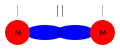
\includegraphics[width=0.6\textwidth]{AFM2.pdf}
            \caption{Darstellung zur Veranschaulichung der antiferromagnetischen Kopplung.
            Als Ligand fungiert hier ein Sauerstoffatom mit seinem p-Orbital (blau).
            Die Spins der d-Orbitale der Metalle (rot) koppeln ferromagnetische mit denen des Sauerstoffs.
            So entsteht die antiferromagnetische Kopplung der beiden Metallatome.}
            \label{fig:AFM}
        \end{figure}
        Ursache des Antiferromagnetismus ist der Superaustausch.
        Beim Superaustausch koppeln zwei Atome mit einem magnetischen Moment über ein weiteres nicht magnetische Atom. 
        Dabei kann die Kopplung ferro- oder antiferromagnetisch sein, meist jedoch antiferromagnetisch \cite{AFM_1}.
        Sind die beiden koppelnden magnetischen Momente nicht gleich groß, so tritt Ferrimagnetismus auf, es gibt dann eine makroskopische Magnetisierung.
        Der Superaustausch ist winkelabhängig, da es dabei um den Überlapp der Orbitale geht.
        Für die Erklärung wird sich hier nur auf die \SI{180}{\degree} Wechselwirkung beschränkt.
        Beispielhaft ist die Kopplung in \autoref{fig:AFM} dargestellt.
        Es kommt bei diesem indirekten Austausch nicht zu einem Überlapp der spintragenden Wellenfunktionen sondern zu der Vermittlung der langreichweitigen Ordnung über einen Liganden.
        Direkter Austausch sorgt für ferromagnetische Kopplung benachbarter andersartige (nicht magnetische) Atome.
        Zwischen Metall und Ligand herscht also direkte Austauschwechselwirkung und damit eine indirekte Austauschwechselwirkung, der Superaustausch zum übernächsten Atom, einem weiteren Metallatom.
        Bei den vorliegenden Metalloxiden ist es so, dass die Elektronen der Metallatom des nicht vollen 3d Oribtals über die 2p Orbitale des Sauerstoffs koppeln.
        Da dieses Orbital voll ist, müssen die Elektronen unterschiedliche Spinrichtung haben.
        Damit besitzten die Sauerstoffatome auch kein eigenes magnetisches Moment.
        Somit ist dann die Wechselwirkung über das Sauerstoffatom hinweg dann antiferromagnetisch.
        Es ergeben sich so zwei Untergitter, welche unterschiedlicher Spinrichtung sind, die Gesamtmagnetisierung ist also wie für Antiferromagneten erwartet Null.
        % Die Wellenfunktionen der Kationen überlappen nur gering und da die Austauschwechselwirkung nur geringe Reichweiten hat können nur die 3d und 2p überlappen.
        % \begin{itemize}
        %     \item Magnonen
        % \end{itemize}
        
        Die Anwenungen des Antiferromagnetismus ist zum Beispiel der nutzen als \textit{Pinning}-Lage, die in spinelektronischen Bauteilen die Orientierung einer ferromagnetischen Schicht festlegt.
        
            
    
    \section{Wechselwirkung von Oberfläche mit Molekülen}
        Moleküle haben im Gegensatz zu Festkörpern, energetisch separierte Zustände, die Orbitale.
        Werden Molekül auf eine Oberfläche aufgebracht so kommt es zur Wechselwirkung zwischen diesen und der Struktur der Oberfläche.
        Bei der Wechselwirkung von Molekülen mit Oberflächen wird in zwei Arten der Adsorption unterschieden. 
        Zum Einen der Physisorption und der Chemisorption, welche wiederum in stark und schwach unterschieden wird.
        Zwischen den beiden Adsorptionsarten lässt sich durch ihre Bindungsstärke von den Molekülen auf dem Substrat unterscheiden.
        Dabei wird als Bindungsstärke die Energie bezeichnet, die nötig ist um ein Molekül von der Oberfläche zu lösen.
        In beiden Fällen handelt es sich um eine Adsorption die auch die Oberflächenstruktur des Substrates beeinflussen können.
        So können neue Zustände entstehen und vorhandene Eigenschaften stark verändert werden.
        %~\cite{ma-DJ
        
        \subsection{Physisorption}
            Bei der Physisorption spielt maßgeblich die Van-der-Waals-Kraft eine Rolle, hat also eine eher geringe Bindungsenergie der Moleküle zum Substrat~\cite{cinchetti_activating_2017}.
            Charakteristisch für die Physisorption ist die Abwesenheit von chemischen Bindungen sowie einen Substrat-Adsorbat-Abstand von mehr als \SI{3}{\angstrom}. %~\cite{bergenti_spinterface_2019}
            Da die Wechselwirkung bei der Physisorption nur gering ist werden die Eigenschaften der Oberfläche und des Moleküles nur schwach beeinflusst~\cite{bergenti_spinterface_2019}.
            Allerdings kann es beim Substrat zu Relaxation kommen.
            Die Bindungen des Moleküls werden nur schwach beeinflusst, sodass sie den Eigenschaften aus der Gasphase stark ähneln~\cite{cinchetti_activating_2017}.
            Die Van-der-Waals-Kraft gehört zu den elektrostatischen Kräften, es werden also keine Elektronen mit dem Substrat ausgetauscht~\cite{bergenti_spinterface_2019}.
            Allein die Induzierung und Fluktuation von Dipolen führt zu dieser Bindung zwischen Molekül und Substrat.
            Die Van-der-Waals-Kraft kann man in drei Arten unterteilen:
            \begin{itemize}
                \item \textbf{Dipol-Dipol-Kraft:} Sie ist die Kraft zwischen zwei permanenten Dipolen, die Keeson-Wechselwirkung.
                \item \textbf{Dipol-induzierter-Dipol-Kraft:} Die Wechselwirkung zwischen einem induziertem Dipol und einem Dipol wird auch als Debye-Wechselwirkung bezeichnet.
                \item \textbf{Londonsche Dispersions-Wechselwirkung:} Zwischen zwei induzierten Dipolen wirkt die Londonsche Dispersions-Wechselwirkung, sie dominiert meist die Van-der-Waals Kraft.
            \end{itemize}

            Die Physisorption kann durch zwei Potetiale beschrieben werden.
            Das eine Potential wirkt repulsiv und resultiert aus dem Pauliverbot.
            Kommen sich Molekülorbital und Substratorbital zunah, überlappen diese.
            Auf Grund des Pauliverbots dürfen keine zwei Elektronen dann in allen Quantenzahlen übereinstimmen und es resultiert in eine abstoßende Kraft.
            Attraktives Potentential resultiert dabei aus der Debye-Wechselwirkung.
            So kommt es beim Gleichgewicht zu einem stabilen Substrat-Molekül-Abstand.
            Das gesamtpotential ist auch als Lennard-Jones-Potential bekannt.
            Vermehrt tritt die Physisorption bei Halbleitern und Isolatoren auf, da die Molekülzustände in der Bandlücke liegen und so keine Bindung mit dem Substrat eigegangen werden kann~\cite{IF_1}.
        
        \subsection{Chemisorption}
            % Im Gegensatz zur Physisorption findet bei der Chemisorption  ein Austausch von Elektronen stattfinden.
            Im Gegensatz zur Physisorption sind die Bindungen um Einiges stärker und führen somit zu Veränderung am Substrat wie auch den Molekülen~\cite{bergenti_spinterface_2019}.
            Ferner wird von Chemisorption gesprochen, wenn die Stärke der Wechselwirkung größer als \SI{1}{\electronvolt} ist~\cite{muscat_chemisorption_1978}.
            Aber dies allein ist nicht ausschlaggebend, es muss eine chemische Veränderung auftreten.
            Dabei kann es sich um kovalente und ionische Bindungen handeln und es kann zum Ladungsaustausch und/oder Hybridisierung kommen~\cite{harutyunyan_hybridisation_2013}.
            Beim Ladungsaustausch kann ein zunächst unbesetztes Orbital unter die Fermikante rutschen und besetzt werden, es kann also neben den strukturellen auch zu elektronischen Veränderungen kommen.
            Im Gegensatz dazu können bei der Hybridisierung mehrer Zustände vom Molekül und/oder Oberfläche durchmischt werden.
            Verbreiterungen, Verschiebungen und auch Aufspaltungen von Molekülzuständen kann die Folge sein~\cite{IF_1}.

            \begin{figure}
                \centering
                \includegraphics[width=0.6\textwidth]{Chemisorption2.PNG}
                \caption{Das adsorbierte Molekül hybridiziert mit dem s-/p-Band des Substartes (1), der schwachen Chemisorption.
                In einem weiteren Schritt kommt es dann zur starken Chemisorption durch Einbindung der d-Bänder (2, oben), es entsteht ein bindendes und ein antibindenes Orbital.
                Durch die Lage der d-Bänder werden nun das bindenden und antibindendene Orbital besetzt, dadurch kommt es zu einer repulsiven Kraft und die Bindung wird wieder geschwächt (unten). Aus~\cite{IF_1}.}
                \label{fig:Chemisorption}
            \end{figure}
            Schwache Bindungen werden meist durch die Wechselwirkung mit den breiten s- oder p-Bändern hervorgerufen.
            Wodurch sich das Energieniveau der Moleküle absenkt und verbreitert, siehe dazu in \autoref{fig:Chemisorption}.
            Für die starke Chemisorption folgt ein weiterer Schritt, der nun abgesenkte Zustand überlappt mit dem der näherungsweise d-Bänder.
            Es bilden sich bindende und antibindendene Zustände aus.
            Ja nach Lage des Ferminiveaus wird nur der bindenden Zustand (starke Adsorption) oder auch (nur teilweise) der antibindene Zustand gefüllt, wodurch repulsiv Kräfte auftreten.
            Ferner beeinflusst auch die Ausdehnung der d-Bänder die Stärke der Chemisorption.
        
        \subsection{Selbstanordnung}
            \begin{figure}
                \centering
                \includegraphics[width=0.6\textwidth]{Adsorbate}
                \caption{Die Adsorbateplätze für verschieden orientierte Oberflächen eines flächenzentrierten Kristalls.
                Es gibt Plätze direkt oberhalb eines Substratatoms (\textit{on top} - t).
                Zwischen zwei Substratatomen gibt es kurze (b) und lange (b') Brückenplätze (\textit{bridge}), sowie Muldenplätze hexagonaler dicht gepacktester Struktur (\textit{hollow} - h) und flächenzentrierter Struktur (h'). Aus~\cite{Fauster}.}
                \label{fig:Adsorbate}
            \end{figure}
            Einige Moleküle ordnen sich regelmäßig auf dem Substrat an, dieser Effekt wird Selbstanordnung genannt.
            Dabei bilden die Moleküle eine Überstruktur im Vergleich zum Gitter des Substrates.
            Gewünscht ist dies, da dann die Molekül einheitlich auf der Oberfläche orientiert sind und somit auch ihre Orbitale, dies ist notwendig für die Molekülorbital-Tomographie (s. \autoref{sec:MOT}).
            Ferner lassen sich gitteratig verteilte Moleküle gezielter manipulieren, wie es für Anwendungen notwendig ist.
            
            Moleküle stellen eine Art der Adsorbate da und können sich an verschiedene Stellen des Substrates setzen.
            Hier wird auf drei unterschiedeliche Möglichkeiten unterschieden dem Platz direkt über einem Substratatom (\textit{on top}), zwischen zwei Substratatomen (\textit{bridge}) oder in der Mitte von mehreren Substratatomen in einer Mulde (\textit{hollow}).
            Beispielhaft ist dies für einen flächenzentrierten Kristall mit verschiedenen Oberfläche in \autoref{fig:Adsorbate} dargstellt.
            Die physikalische Ursache ist noch nicht ganz klar, warum sich manche Moleküle auf einigen Substraten ordnen und andere hingegen nicht.
            Naheliegend ist, dass es mit der Wechselwirkung zusammenhängt und der Affinität Elektronen auszutauschen.
            Dies wurde bereits auf die Austrittsarbeit für einige Metaloxide hinweg untersucht \cite{greiner_universal_2012}.

            Das Wechselspiel zwischen der Molekül-Molekül-Wechselwirkung und Molekül-Substrat-Wechselwirkung definiert die finale Struktur \cite{IF_1}.
            Dabei sind vor Allem gerichtete Kräfte wichtig um die Regelmäßigkeit zu erhalten.
            Schwächste und ungerichteste Kraft ist die Van-der-Waals-Kraft, genauer die Debye-Wechselwirkung (\SIrange{0.02}{0.1}{\electronvolt}), die allerdings sehr langreichweitig ist.
            Weitere Ursache ist der Einfluss des Substrates auf die Wechselwirkung den Molekülen untereinander, z.B. durch Oszillationen des Oberflächenpotentials.
            Die Keeson-Wechselwirkung als Ursache der Dipol-Dipol-Interaktion hat ebenfalls Beteiligung an der Anordnung der Moleküle, allerdings nur wenn die Moleküle ein permanetes Dipolmoment haben.
            Mit der Wasserstoff-Brücken-Bindung (\SIrange{0.01}{1.73}{\electronvolt}) unter den Molekülen bindet sich ein Wasserstoffatom an ein elektronegativeres Atom, hierdurch kommt es zu Ladungsverschiebung innerhalb der Bindung.
            Das positivere Wasserstoffatom kann nunmehr eine elektrostatische Bindung zu einem weiteren Atom einnehmen.
            Wasserstoff-Brücken-Bindungen sind je stärker sie werden eher geradlinig gerichtete Bindungen mit einer kurzen Bindungslänge.
            Metallisch Koordination ist eine weiter Form der Bindung (\SIrange{0.5}{2}{\electronvolt}), die Moleküle funkieren als Linker zwischen einzelenen Metallatomen.
            Die stärkste und gerichteste Kraft ist jedoch die kovalente Bindung, welche gleichzeitig auch die elektronische Struktur stark beeinflusst.
            Sie ist sogar so stark, dass sie teilweise eine perfekte Selbstanordnung behindert und damit eher zu weniger geordneten Strukturen führen kann \cite{IF_1}.

            Neuste Studien zeigen, dass die Energieniveauanpassung maßgeblich durch die Austrittsarbeit beeinflusst wird \cite{IF_3}.
            Hierzu wurden verschiedene Metaloxide untersucht mit dem Ergebnis, ...

        \subsection{Energieniveau-Anpassung}
            Für die Anwendung besonders bedeutsam ist die Energieniveau-Anpassung, welche Einfluss auf den Elektronen- und Lochtransport hat~\cite{IF_4}.
            Bei Metalloxiden verschiebt sich durch die Austrittsarbeit die relative Position des Valenz- und Leitungsbandes zum Vakuumniveau \cite{IF_3}.
            Die meisten der Metalloxide haben keine besetzten Zustände nahe der Fermikante, da diese in eine Bandlücke fällt.
            Folglich ist auch Ladungsübertrag vom Substrat auf die Moleküle nur vom Valenz- oder Leitungsband aus möglich.
            Auch wenn einige Oxide Ladungsaustausch zwischen Valenzband und dem höcsten bestzten Molekülorbital (HOMO, \textit{highest occoupied molecular orbital}) zulassen so  gibt es noch kein Model, dass dies beschreibt.
            Verbreitet ist jedoch der Ansatz der Ferminiveau-Anheftung für nicht reaktive Grenzflächen zwischen Molekülen und Oxiden.

            Greiner u.a. \cite{IF_3} fanden heraus, dass die Bandstruktur des Substartes dabei nur eine untergeordnete Rolle spielt.
            Ausschlaggebend für die Energieniveau-Anpassung ist das elektrochemische Potential des Substrates mit dem Reduktionspotentials des Moleküls.
            Genauer die Differenz zwischen der Austrittsarbeit des Substrates und der Ionisationsenergie.
            Als Ionisationsenergie wird die Energie zwischen höchsten besetztem Molekülorbital und dem Vakuumlevel verstanden.
            Die Elektronenaffinität entspricht der Energie zwischen dem Vakuumlevel und dem niedrigsten unbestzten Molekülorbital (LUMO, \textit{lowest unoccoupied molecular orbital}).

            Auch bei Isolatoren kann sich ein Oberflächendipol ausbilden.
            Wegen des Pauliverbot und den zusätzlichen Elektronen der Moleküle an der Grenzfläche werden die Elektronen an der Oberfläche in den Festkörper zurück gedrenkt.
            Durch die Unabhängigkeit vom Adsorptionstyp tritt dieser \textit{Push-Back}-Effekt immer auf~\cite{IF_4} und reduziert damit das Oberflächendipolmoment~\cite{IF_1}.
            Zusätzlich kann das Oberflächendipolmoment durch Ladungsaustausch zwischen Molekül und Substrat geschwächt oder andersherum gestärkt werden.
            Hinzukommend gibt es gegebenfalls noch einen permanenten Dipol des Moleküls, welcher beachtet werden muss.

            \begin{itemize}
                \item charge transfer from HOMO to Ef? \cite{IF_4}
                \item \textbf{Ferminiveau Anheftung}
            \end{itemize}


    \section{Substrate und Molekül Eigenschaften}
        \subsection{Nickeloxid (111) Oberfläche}
            \begin{figure}
                \centering
                \includegraphics[width=4cm]{NiO/NiO-structure.jpg}
                \caption{Die Krsiatllstruktur von Nickeloxid. Das $\ce{Ni}^{2+}$ Ion befindet sich in einer oktaedrischen Umgebung von $\ce{O}^{2-}$ Ionen. Aus~\cite{NiO-structure}.}
                \label{fig:NiO-structure}
            \end{figure}
            Nickeloxid besitzt die Struktur von \ce{NaCl} und ist in \autoref{fig:NiO-structure} dargestellt~\cite{kunz_chemisorption_1985}.
            Hierbei handelt es sich um ein Monooxid und die Sauerstoffatome sitzen in oktaedrischen Zwischenräumen zwischen den Nickelatomen.
            Die geometrische Gitterkonstante beträgt \SI{4.17}{\angstrom}~\cite{sebbari_uranyl_2012}.
            Für die magnetische Ordnung ergibt sich die dopplte Gitterkonstante zwischen zwei gleich ausgerichteten Spins~\cite{Suter}.
            Die Austrittsarbeit lässt sich dabei durch die Präperation beeinflussen und liegt zwischen \SIrange[range-phrase=' und ']{4.5}{5.2}{\electronvolt} \cite{poulain_electronic_2020}.
            % Neutronenbeugung auf Spin empfindlich also dopplte Einheitszelle, anders als die chemisch empfinliche Röntgenbeugung.

            Nickeloxid gehört zu der Familie der Antiferromagneten mit einer Neél-Temperatur von \SI{525}{\kelvin}.
            Da das 3d Band des Nickels im Oxid nur teilweise gefüllt ist (acht von zehn möglichen Elektronen) würde man erwarten, dass es sich hierbei um einen Leiter handelt~\cite{kunz_chemisorption_1985}.
            Dies ist allerdings nicht so und Nickeloxid ist ein Isolator, genauer ein Ladungs-Transferisolator.
            Die thermische Bandlücke liegt bei \SI{3.6}{\electronvolt}~\cite{kunz_chemisorption_1985}.

            Ein Oberflächendipolelement ist besonders stark in der (111)-Orientierung ausgeprägt, da bei der polaren Oberfläche entweder nur Sauerstoff oder nur Nickelionen in der obersten Lage vorhanden sind~\cite{NiO_8}.
            Dies liegt an der Bindung zwischen dem Sauerstoff und dem Nickel.
            Das Oberflächenpotential ist folglich divergent und somit die Oberfläche instabil.
            Problematisch an dünnen Filmen von Nickeloxid in der (111)-Orientierung ist diese Instabilität und die starke Abhänigkeit vom Präperationsprozess \cite{NiO_36}.
            Es gibt verschiedene Beobachtungen zu der Stabilisierung der polaren Oberfläche wie die Rekonstruktion oder \ce{OH-}-Terminierung \cite{NiO_36, NiO_35, NiO_34, NiO_27, NiO_10}.
            Bei der Stabilisierung wird die Oberflächenladung reduziert und damit das Oberflächenpotential gesenkt in Folge dessen es zur Ausbildung einer stabilen Oberfläche kommt.

            Die Magnetisierung ist ebenso wie die Atome abwechseln geschichtet.
            So tritt zunächst eine Ebene mit Nickel auf, in der die Magnetisierung antiparallel zu der nächsten Schicht Nickel ist.
            Denn die Spins innerhalb einer (111)-Ebene koppeln ferromagnetisch wohingegen die Kopplung unter den Ebenen antiferromagnetisch ist~\cite{FeO_6}.

            Nickeloxid zeigt bereits für andere Orientierung für einige Moleküle Chemisorption, was durch enthaltene Defekt hervorgerufen wird~\cite{kunz_chemisorption_1985}.
            Auf Grund dessen eignet sich das Substrat zur Untersuchung bestens, zumal für polare Oberflächen auch eine größere Reaktivität vorhergesagt wird \textbf{Quelle}.
            \begin{itemize}
                \item elektronische Struktur
            \end{itemize}

        

        \subsection{Magnetit}
            Das Magnetit ist chemisch gesehen ein Eisenoxid (\ce{Fe3O4}), welches in der inversen Spinellstruktur kristallisiert.
            Die Gitterkonstante beträgt dabei \SI{8.397}{\angstrom}~\cite{springer_database}.
            % und hat damit eine Abweichung um \SI{2.4}{\percent} von der dreifachen Gitterkonstante des Eisens. - Orientierung beachten


        
        \subsection{Eisenmonooxid (100) Oberfläche}
            Ebenso wie das Nickeloxid kristallisiert auch das Eisenmonooxid, welches auch Wüstite genannt wird, in der \ce{NaCl}-Struktur~\cite{FeO_4}.
            \textbf{Dabei beträgt die Gitterkonstante \SI{3.07}{\angstrom}~\cite{FeO_1} - ist da sowas wie Einheitszelle der 100 gemeint}
            Dabei beträgt die Gitterkonstante \SI{4.308}{\angstrom}~\cite{springer_database} und die $\ce{Fe}^{2+}$-Ionen befinden sich einer oktaedrischen Position zum Sauerstoff~\cite{FeO_4}.
            Es handelt sich ebenfalls um einen Isolator mit antiferromagnetischen Eigenschaften und einer Neél-Temperatur von \SI{198}{\kelvin}~\cite{FeO_4}.
            Die Bandlücke wurde dabei auf \SI{2.4}{\electronvolt} bestimmt. \textbf{Wdowik - 2013 - Strong effects of cation vacancies on the electron.pdf}

            Genau wie in Nickeloxid sind auch hier die (111)-Ebenen untereinander antiferromagnetisch gekoppelt.
            So ergibt sich auf der (100)-Oberfläche abwechselnd Spin ausgerichtete
            nicht-stöchiometrische Verbindung wie das Eisenoxid enthalten dabei verschiedene Oxidationszustände also nicht nur Fe2+ sondern auch \SIrange{10}{32}{\percent} Fe3+ \cite{FeO_11}.
            Fe2+ befinden sich in oktaedrischer Umgebung
            O anions and metal cations
            Fe2+ magnetic moments aligned parallel to the close packed (111) planes, but in opposite directions from one plane to the next. The Fe defect clusters discussed above are thought to affect the magnetic properties 

            \begin{itemize}
                \item WKF
                \item Symmetrie - p4mm
            \end{itemize}
            FeO (sog. Wüstit) ist als Hochtemperaturphase nur oberhalb von 560oC stabil.
            Es handelt sich gemäß FexO (x=0.95-0.88) um eine nichtstöchiometrische Verbindung mit Defekten im Kationenteilgitter. \url{http://ruby.chemie.uni-freiburg.de/Vorlesung/metalle_8_5.html}
    

        \subsection{Pentacene} \label{sec:5A}         
            \begin{figure}
                \centering
                \includegraphics[width=0.6\textwidth]{PEN.jpg}
                \caption{Geometrische Struktur des Pentacene sowei die vier höchsten besetzten und vier niedrigesten unbesetzen Orbitale. Vorlage aus~\cite{PEN}.}
                \label{fig:PEN}
            \end{figure}
            Schon häufig wird Pentace als kleines Molekül in elektronischen Bauteilen eingesetzt~\cite{5A_4}.
            Bei Pentacene ($\ce{C22H14}$) oder auch kurz 5A handelt es sich um einen Elektronendonator und gehört zu den p-Typ Halbleiter~\cite{5A_1}.
            Seine Struktur ist in \autoref{fig:PEN} dargestellt, welche sich aus linear an Kanten verschmolzenen Phenylringen zusammensetzt~\cite{MM_2}.
            Ebenfalls zu sehen sind jeweils die ersten vier höchsten besetzen und niedrigesten unbesetzten Zustände.
            Die Synthese des Pentacene ist auf Grund der einfachen Struktur ebenfalls einfach.
            Pentacene bringt die perfekten Eigenschaften für Molekülorbitaltomographie mit, da es sich um ein \pi-konjugiertes Molekül handelt~\cite{MM_2}.
            Ferner weist das Molekül keinen permanenten Dipol auf~\cite{5A_4}.

            In dünnen Filmen aus Pentacene zeigt sich eine hohe Elektronenbeweglichkeit.
            Auf der Gold(111)-Oberfläche ordnet es sich an und liegt parallel zum Substrat.
            Der Abstand zwischen den Molekülen und Substrat wird auf \SI{3.28}{\angstrom} bestimmt, was auch in der Größenordnung für Physisorption liegt~\cite{5A_1}.
            

            Dichte von \SI{1.232(6)}{\gram\per\cubic\centi\meter}~\cite{CAS}.

            \section{IDEEN}
            \begin{itemize}
                \item O1s erklären
                \item Fe3p erklären 
                \item XMLD
                \item XPS ausführlicher? (Asymmetrie)
                \item Kreios mit Blenden überarbeiten?
                \item Übergangsmetalloxide
                \item mehr Motivierend aktuelle Anwendung
            \end{itemize}
            